\section{Alternativmethode}
\label{sec:alternativ}
Bei der Alternativmethode haben wir uns für den k-nächste Nachbarn (KNN) Algorithmus entschieden.
Diesem übergeben wir drei Features die wir vorerst generieren.
Die drei Features sind pro Bild der Mittelwert der Pixelwerte, die Standardabweichung der Pixelwerte und der Mittelwert der Norm des Gradienten der Pixelwerte.
Wir haben uns dabei gedacht, dass durch den Mittelwert und die Standardabweichung erkannt werden kann ob ein Bild gleichmäßig in seiner Farbwahl ist oder nicht.
Durch den Mittelwert der Norm des Gradienten wollten wir ein Maß für die Stärke der Farbänderung haben.
Mit diesen drei Features trainieren wir den KNN auf den "Undersampling" Trainingssatz, da für das Trainieren mit den "Oversampling" Trainingsdaten die Rechenleistung nicht ausreichte.
Zudem denken wir, dass es für den KNN nicht Vorteilhaft gewesen wäre mit Daten zu trainieren die sich teilweise doppeln, da Dopplungen perfekte Nachbarn wären.
Der KNN erreicht auf dem "Undersampling" Testsatz folgende Genauigkeit
\begin{align*}
    \text{Genauigkeit} &= 15.00\, \%
\end{align*}
und schneidet damit wesentlich schlechter ab als das CNN.
In Abbildung \ref{fig:alternativ} ist die Konfusionsmatrix des KNN zu sehen.
\begin{figure}
    \centering
    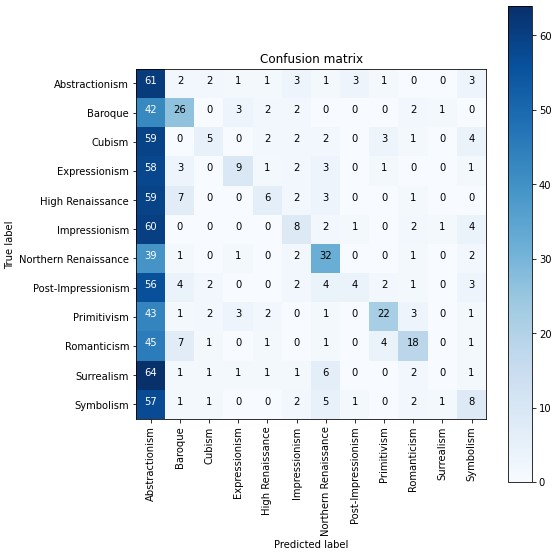
\includegraphics[width=0.5\textwidth]{content/data/alternativ.JPG}
    \caption{Die Konfusionsmatrix des KNN auf den Testdaten.}
    \label{fig:alternativ}
\end{figure}
Wie zu sehen ist sagt der KNN für fast jedes Bild das Genre "Abstrakte Expressionismus" (in der Abbildung "Abstractionism").
Wir sind uns leider nicht sicher, warum der KNN fast nur dieses Genre ausgibt.
Nur auf einigen Genre bestimmt der KNN etwa ein drittel der Bilder richtig.
Am zuverlässigsten tut er dies für die "Niederländische Renaissance" (in der Abbildung "Northern Renaissance"), da diese Bilder im genutzten Datensatz oft nur in scharz-weiß sind.
